% vim: set tw=78 tabstop=4 shiftwidth=4 aw ai:

\chapter{Un tracker overlay BitTorrent inovativ pentru unificare de swarm-uri}
\label{chapter:unified-tracker}

Rolul de tracker BitTorrent și problema acestuia de a fi un singur punct de
eșec, poate fi rezolvată prin folosirea PEX (\textit{Peer Exchange}) și DHT
(\textit{Distributed Hash Table})~\cite{dht-paper}. Aceste tehnologii noi
oferă modalități inovative pentru descoperirea de peer-i, fără a fi necesar un
tracker BitTorrent. Informația de control este transmisă de la un peer la
altul. Majoritatea implementărilor de azi oferă PEX și DHT, cuplate cu
folosirea unui tracker. Spre exemplu, în libtorrent-rasterbar se folosesc în același timp atât date obținute prin DHT cât și printr-un tracker clasic.

Rolul extinderii funcționalității tracker-ului este de a asigura redundanță și pentru a simplifica arhitectura. Prin construirea unui tracker overlay pentru unificarea de swarm-uri se dezvoltă swarm-ul, asigurându-se prezența unui număr mai mare de leecher-i și seeder-i, cu potențialul de a mări viteza acestuia. Deoarece sănătatea unui swarm nu se bazează exclusiv pe numărul de peer-i din acesta ci și pe raportul dintre seeder-i și leecher-i, abordări precum construirea de swarm-uri private sau asigurarea moderării sunt importante. Aceste abordări asigură o bază pentru extinderea disponibilității seeder-ilor dintr-un swarm și pentru un flux constant de date.

Tracker-ele sunt exclusiv entități server. Sunt contactate de peer-i pentru
actualizarea informației interne și returnează informație acestora. Baza de
date a tracker-elor stochează informații despre peer-i care fac parte din
swarm, cât și date statistice legate de aceștia, cum ar fi cantitatea de
informație descărcată. Această informație a fost folosită intens de Bardac~et~al~\cite{tracker-mon} pentru construirea unui serviciu de monitorizare a tracker-elor. Propunerea noastră este de a extinde mesajele existente ale tracker-elor pentru a le permite acestora să se interconecteze -- adică să comunice unul cu altul, pe lângă comunicația existentă cu peer-ii din swarm.

\section{Context și obiective}
\label{sec:unified-tracker:context}

Ne propunem să tratăm problema unificării unor swarm-uri separate, care iau
parte într-o sesiune în care se partajează același fișier. Propunem un
protocol de unificare de tracker-e care permite unor swarm-uri diferite, ce
folosesc fișiere .torrent diferite, să conveargă. Se definește unificarea de
swarm-uri posibilitatea clienților din diferite swarm-uri să comunice unul cu
celălalt. La baza unificării stă un ,,protocol de convergență centrat pe
tracker'' prin care tracker-e dintr-o rețea de overlay își trimit informații despre peer-i unul altuia.

Obiectivul protocolului de unificare de swarm-uri este integrarea de peer-i care fac parte din alte swarm-uri și partajează același fișier. Aceste swarm-uri, numite \textit{swarm-uri comune}, partajează același conținut, dar au tracker-e diferite.

Am proiectat o rețea overlay de tracker-e care le permite acestora să partajeze informație și să integreze peer-i în swarm-urile respective. Overlay-ul se bazează pe Tracker Swarm Unification Protocol (TSUP), care permite notificări de actualizare și livrare de informție tracker-elor din overlay. Arhitectura protocolului este inspirată din protocoalele de rutare din rețelele de calculatoare.

Protocolul propus în acest articol, numit \textbf{Tracker Swarm Unification Protocol (TSUP)}, face posibilă unificarea de swarm-uri care partajează aceleași fișiere, utilizând o rețea overlay de tracker-e. Un tracker care are implementat acest protocol va fi numit aici \textbf{tracker unificat}.

\begin{figure}[h]
  \begin{center}
    \includegraphics[width=0.7\textwidth]{src/img/unified-tracker/unified-trackers}
  \end{center}
  \caption{Unified trackers}
  \label{fig:unified-tracker:unified-trackers}
\end{figure}

Fișierele torrent create pentru același conținut au același
\textit{info_hash}; așadar în swarm-uri care partajează aceleași fișiere
(swarm-uri comune), peer-ii vor anunța către tracker același
\textit{info_hash}. De aceea tracker-ele care implementează TSUP pot ,,unifica'' aceste swarm-uri comune, comunicând unul cu celălalt pentru a schimba informație despre peer-i care contribuie la partajarea acelorași fișiere, cu același \textit{info_hash}. Pentru a realiza acest lucru, tracker-ele unificate își trimit actualizări periodice, care conțin informații despre peer-ii din rețea.

\section{Protocolul de unificare a swarm-urilor}
\label{sec:unified-tracker:swarm-unification}

Așa cum s-a menționat mai sus, \textit{TSUP} este acronimul de la \textit{Tracker Swarm Unification Protocol}. TSUP este responsabil cu comunicația dintre tracker-e, pentru schimbul de informații despre peer-i în swarm-uri comune.

Pentru nivelul transport al comunicației, protocolul folosește UDP (User
Datagram Protocol) pentru a reduce consumul de resurse. Un tracker are deja de
procesate mai multe conexiuni TCP (Transport Control Protocol) cu alți peer-i; adăugând conexiuni TCP suplimentare către fiecare din tracker-ele vecine ar crește prea mult încărcarea pentru un overlay mare de tracker-e. Mesajele schimbate de la un tracker la altul nu au nevoie de controlul fluxului oferit de TCP și au nevoie un nivel mai scăzut de fiabilitate decât cel oferit de TCP, așa cum va fi explicat în continuare. Simplitatea protocolului UDP oferă așadar avantajele unei comunicații cu mai puține bătăi de cap.

În TSUP pot fi identificate următoarele procese:
\begin{itemize}
    \item \textbf{Procesul de stabilire a conexiunilor virtuale:} Un
    three-way-handshake responsabil cu stabilirea unei ,,conexiuni'' UDP la nivelul aplicație între două tracker-e. Procesul este demarat de un pachet \textit{SYN} (Synchronization Packet).
    \item \textbf{Procesul de unificare:} Tracker-ele schimbă pachete de
    unificare, numite pachete \textit{SUMMARY}, printr-un three-way-handshake, pentru a afla care sunt swarm-urile comune.
    \item \textbf{Procesul de actualizare:} Tracker-ele fac schimb de peer-i din swarm-uri comune prin pachete \textit{UPDATE}.
    \item \textbf{Procesul electoral:} Stabilirea unui \textit{leader de swarm} responsabil cu primirea tuturor actualizărilor de la tracker-ele legate vecine, agregarea acestor actualizări și trimiterea rezultatului agregat înapoi la acestea.
\end{itemize}

\textit{Procesul de unificare} include un process de actualizare în three-way-handshake-ul său, astfel încât cele două operații, unificare și actualizare, sunt realizate în pipeline. De fiecare dată când un nou fișier torrent se înregistrează la tracker, un nou swarm este creat. Un proces de unificare este declanșat și un pachet SUMMARY este trimis imediat către fiecare tracker vecin, informându-l de noul swarm.

\textit{Procesul de actualizare} este declanșat periodic, astfel încât pachetele de actualizare (UPDATE) sunt trimise la un interval configurabil de timp la fiecare tracker din swarm-ul comun. Valoarea implicită pentru trimiterea pachetelor UPDATE este de 30 de secunde.

Pentru menținerea conexiunilor virtuale dintre tracker-e, se trimit periodic pachete HELLO, care acționează ca un mecanism de tip keep-alive. Valoarea implicită pentru trimiterea pachetelor HELLO este de 10 secunde, dar valoarea poate fi schimbată din configurația protocolului, Dacă niciun pachet HELLO nu este primit într-un interval configurabil, numit interval de deconectare, conexiunea virtuală este întreruptă și un nou proces de stabilire a conexiunii virtuale este început pentru acea legătură, trimițând un pachet SYN.

Comunicația dintre tracker-e este condiționată de cunoașterea acestora. Pentru a realiza acest lucru, în versiunea curentă a protocolului, fiecare tracker este configurat static cu o listă de alte tracker-e cu care trebuie să se realizeze comunicația. Fiecare element din listă reprezintă o \textit{legătură} identificată printr-un host name (URL sau adresă IP) și un port. Și alți parametri pot fi configurați pentru legătură, unii dintre ei pot fi specifici implementării. Dacă procesul de stabilire a conexiunii virtuale reușește, legătura devine o conexiune virtuală, care este menținută de pachete keep-alive (pachete \textit{HELLO}).

Pentru a îmbunătăți scalabilitatea TSUP, tracker-ele pot fi grupate împreună în \textbf{rețele de tracker-e}. Conexiunile din toate rețelele de tracker-e sunt complete (full mesh). Două rețele de tracker-e sunt conectate prin \textbf{border trackers}.

Penru a configura o topologie care conține mai multe rețele de tracker-e, fiecare legătură către fiecare tracker vecin trebuie să fie setată ca \textbf{legătură internă} sau \textbf{legătură externă}. Tracker-ele conectate cu legături interne fac parte din aceași \textit{rețea de tracker-e}; tracker-ele conectate cu legături externe fac parte din alte rețele. Extrapolând, cele din prima categorie pot fi clasificate ca aparținând unei \textbf{rețele interne}, iar cele din a doua categorie, ca aparținând  unei \textbf{rețele externe}.

Un graf complet care folosește legături interne ca muchii este o \textit{rețea internă}. Un graf complet care folosește legături externe ca muchii este o \textit{rețea externă}. Un tracker care are atât legături interne cât și externe este un border tracker. Informația despre peer-i recepționată dintr-o rețea internă este provenită de la \textbf{peer-i interni}, în timp ce informația recepționată dintr-o rețea externă își are originea la \textbf{peer-i externi}.  Legăturile dintre tracker-e aflate în aceași rețea, indiferent dacă sunt interne sau externe, trebuie să fie complete (full mesh).

Pentru a avea o comunicație scalabilă și care consumă puține resurse, tracker-ele sunt organizate în grupuri în funcție de swarm-ul unificat. Așadar un tracker poate să aparțină în mai mult de un singur grup în același timp. Numărul de grupuri în care aparține este egal cu numărul de swarm-uri de pe tracker-ul respectiv. Fiecare grup conține un \textbf{swarm leader} responsabil cu trimiterea de actualizări către ceilalți membri din grup. Ceilalți membri din grup, în loc să trimită actualizări către vecini pe un graf complet (full mesh), trimit actualizări \textbf{swarm leader}-ului pe un graf de tip arbore reducând încărcarea rețelei la actualizare. Aceste actualizări se propagă la alți peer-i din grup.

Gruparea tracker-elor în rețele crește scalabilitatea systemului, dar, ca un dezavantaj, crește și timpul de convergență. Timpul de acutualizare pentru border trackers poate fi setat la o valoare mai mică pentru a grăbi convergența. Administratorul de sistem trebuie să opteze între convergență și scalabilitate și să adapteze parametrii protocolului la topologie.

\section{Configurația experimentală}
\label{sec:unified-tracker:setup}

Activitățile de testare pentru TSUP au folosit o infrastrucutură virtuală și o platformă de testare peer-to-peer rulată deasupra acesteia. Am desfășurat scenarii care au în componență diverse swarm-uri, de la 4 peer-i și un tracker per swarm, până la 48 de peer-i și 12 tracker-e. Pe lângă testarea și evaluarea în această formă, infrastructura a fost folosită pentru a compara rețeaua overlay de tracker-e cu un swarm clasic care folosește un singur tracker dar același număr de peer-i. Vom arăta că un swarm unificat are o performanță similară în comparație cu un swarm (clasic) cu un singur tracker.

Experimentele au folosit o versiune modificată de hrktorrent, o aplicație cu consum redus de resurse construcită peste libtorrent-rasterbar. Alte experimente desfășurate în trecut~\cite{bt-vi} au arătat că libtorrent-rasterbar depășește alți clienți BitTorrent, acest lucru ducând la decizia noastră de a îl folosi aici. Experimentele desfășurate de noi au folosit o limitare de bandă tipică conexiunilor ADSL+ (viteză de download de 24 Mbit și viteză de upload de 3 Mbit).

\begin{figure}[h]
  \begin{center}
    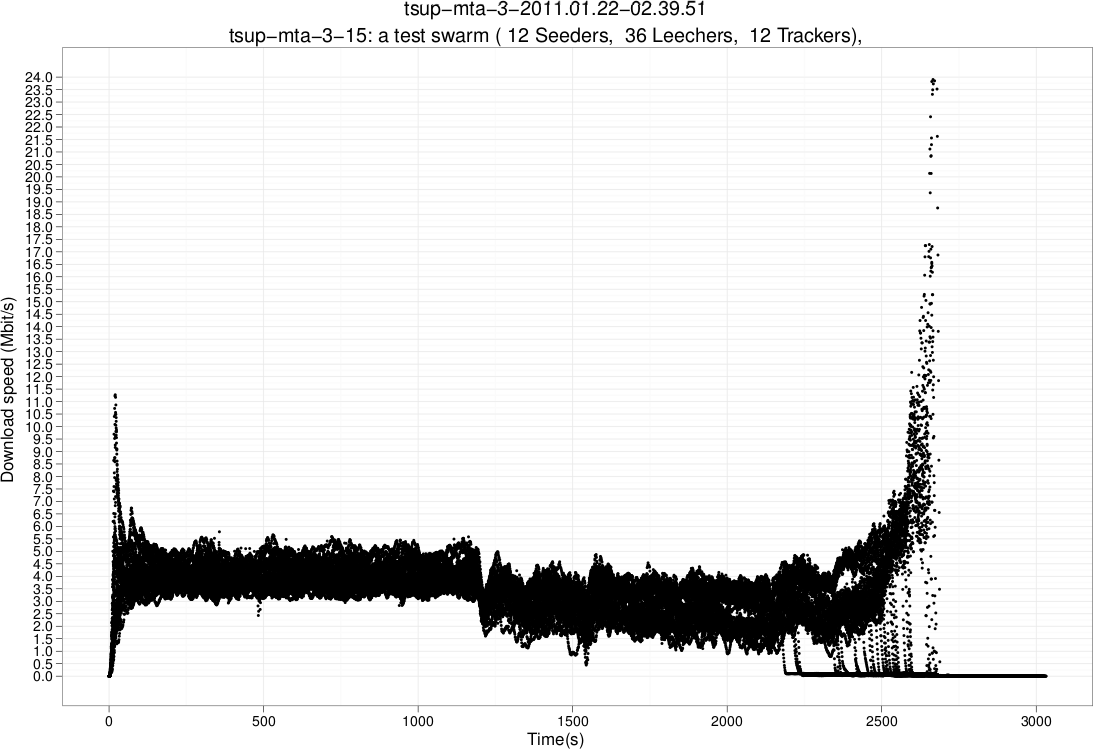
\includegraphics[width=0.7\textwidth]{src/img/unified-tracker/tsup-sample-run-48peers}
  \end{center}
  \caption{Sample Run Graphic}
  \label{fig:unified-tracker:tsup-sample-run}
\end{figure}

O mostră de figură de ieșire generată automat, care descrie o sesiune cu 48 de peer-i (12 seeder-i, 36 leecher-i, 12 tracker-e) partajând un fișier de 1024 MB este ilustrată în Figura~\ref{fig:unified-tracker:tsup-sample-run}. Imaginea arată evoluția vitezei de download pentru toți peer-ii din swarm. Toți sunt limitați la viteza de download de 24 Mbit și viteză de upload de 3 Mbit.

\section{Rezultatele experimentale și evaluarea}
\label{sec:unified-tracker:results}

Pentru a testa efortul suplimentar adăugat de TSUP la protocolul BitTorrent, am desfășurat un set de scenarii care compară viteza medie de download pentru un swarm cu tracker-e unificate cu un alt swarm care are doar un tracker neunificat, dar același număr de leecher-i și seed-eri. Fiecare scenariu de testare este caracterizat de mărimea fișierului partajat, numărul de peer-i și, în cazul testelor cu tracker-e unificate, de numărul de tracker-e de acest tip. Am partajat fișiere de trei mărimi: 64 MB, 256 MB și 1024 MB.

În scenariile de testare cu tracker-e unificate am testat swarm-uri cu 1, 2, 4, 8 și 12 tracker-e. La fiecare tracker au fost conectați 4 peer-i, din care 1 este seeder și 3 sunt leecher-i. Așadar, spre exemplu, într-un scenariu cu 8 tracker-e sunt 8 seeder-i și 24 leecher-i, totalizând 32 de peer-i. Având 3 fișiere și 12 tracker-e în cel mai mare scenariu, a fost necesar să creăm 36 de fișiere .torrent, deoarece pentru fiecare fișier partajat este necesară crearea unui fișier .torrent pentru fiecare tracker. În scenariile corespunzătoare cu tracker-e neunificate există un singur fișier .torrent pentru fiecare fișier partajat. Am variat numărul de seeder-i și leecher-i conectați la tracker astfel încât numărul acestora să fie același cu cel din scenariul corespunzător cu tracker-e unificate.

Rezultatele pot fi văzute în Tabelul~\ref{tab:unified-tracker:comparison}, care arată rezultatele pentru fiecare mărime de fișier, în partea de sus (64 MB), în partea de mijloc (256 MB) și respectiv în partea de jos a tabelului (1024 MB). Pentru fiecare situație dintre acestea, este ilustrată viteza medie de download și deviația standard relativă. În partea din dreapta este ilustrată scăderea de performanță i.e. procentul cu care scade viteza de download în urma urma efortului suplimentar adăugat de TSUP. În partea din stânga a tabelului este ilustrat numărul de seeder-i și leecher-i pentru fiecare scenariu.

Toate valorile pozitive pentru procentele de sub antetul de scădere a performanței marchează o diminuare a performanței cauzată de efortul suplimentar adăugat de TSUP în BitTorrent. O valoare negativă pentru scăderea vitezei de download arată că a avut loc o creștere de performanță în locul unei scăderi.

Procesul de unificare care are loc în XBT Unified Tracker introduce un efort suplimentar în protocolul BitTorrent în comparație cu XBT Tracker. Teoretic, scăderea de performanță ar trebui să fie mereu pozitivă. Dar există situații în care procentele sunt negative, lucru care ar putea sugera faptul că TSUP crește viteza, reducând timpul de download. Dar această creștere de performanță nu se datorează TSUP ci este cauzată de alt factor. În toate scenariile cu un singur tracker, la începutul lor, toți peer-ii sunt porniți aproape simultan, creându-se un flash crowd.  În această situație, comunicația dintre peer-i va începe imediat, dar când mai multe tracker-e sunt unificate, protocolul TSUP impune o latență, justificată de timpul în care un peer află de toți ceilalți, adică timpului de convergență. Se știe că uneori este mai bine atunci când anumiți peer-i intră mai târziu în swarm~\cite{bt-analysis}, explicând prezența acestor valori negative pentru câmpul de scădere a performanței.

\def \singlesods {337.73}
\def \singlestds {472.27}
\def \singlesfds {475.13}
\def \singleseds {476.10}
\def \singleswds {470.53}
\def \singlesorsd {1.28}
\def \singlestrsd {0.87}
\def \singlesfrsd {1.87}
\def \singlesersd {6.06}
\def \singleswrsd {9.61}

\def \singletods {358.72}
\def \singlettds {476.59}
\def \singletfds {477.56}
\def \singleteds {492.40}
\def \singletwds {486.04}
\def \singletorsd {0.45}
\def \singlettrsd {0.26}
\def \singletfrsd {0.45}
\def \singletersd {6.64}
\def \singletwrsd {8.33}

\def \singleoods {365.27}
\def \singleotds {477.47}
\def \singleofds {477.54}
\def \singleoeds {423.71}
\def \singleowds {407.71}
\def \singleoorsd {0.19}
\def \singleotrsd {0.15}
\def \singleofrsd {0.18}
\def \singleoersd {6.19}
\def \singleowrsd {4.47}

\def \multiplesods {335.11}
\def \multiplestds {396.55}
\def \multiplesfds {463.42}
\def \multipleseds {497.35}
\def \multipleswds {496.48}
\def \multiplesorsd {2.87}
\def \multiplestrsd {16.64}
\def \multiplesfrsd {12.60}
\def \multiplesersd {11.10}
\def \multipleswrsd {11.48}

\def \multipletods {356.55}
\def \multiplettds {407.55}
\def \multipletfds {477.45}
\def \multipleteds {500.56}
\def \multipletwds {494.93}
\def \multipletorsd {1.07}
\def \multiplettrsd {14.67}
\def \multipletfrsd {10.73}
\def \multipletersd {8.49}
\def \multipletwrsd {12.38}

\def \multipleoods {365.57}
\def \multipleotds {437.09}
\def \multipleofds {466.03}
\def \multipleoeds {418.69}
\def \multipleowds {418.76}
\def \multipleoorsd {0.31}
\def \multipleotrsd {9.12}
\def \multipleofrsd {5.93}
\def \multipleoersd {8.73}
\def \multipleowrsd {6.27}


\begin{sidewaystable}
  \centering
  \caption{Single Tracker vs. Unified Trackers Comparison}
  \label{tab:unified-tracker:comparison}
  \begin{tabular}{@{}rrcccrccc@{}}
    \toprule
       & & \multicolumn{2}{c}{\textbf{Single Tracker}} & &
       \multicolumn{3}{c}{\textbf{Unified
       Trackers}} & \\
    \cmidrule{3-4} \cmidrule{6-8}
      \textit{seeders} & \textit{leechers} & \textit{mean dspeed (KB/s)} &
      \textit{rel.st.dev. (\%)} & & \textit{trackers} & \textit{mean dspeed (KB/s)} &
      \textit{rel.st.dev. (\%)} & \textit{perf. decrease (\%)} \\
    \midrule
      $size = 64MB$\\
      1 & 3 & \singlesods & \singlesorsd & & 1 & \multiplesods &
      \multiplesorsd & 0.78 \\  %01
      2 & 6 & \singlestds & \singlestrsd & & 6 & \multiplestds &
      \multiplestrsd & 16.03 \\  %04
      4 & 12 & \singlesfds & \singlesfrsd & & 4 & \multiplesfds &
      \multiplesfrsd & 2.46 \\  %07
      8 & 24 & \singleseds & \singlesersd & & 8 & \multipleseds &
      \multiplesersd & -4.46 \\  %10
      12 & 36 & \singleswds & \singleswrsd & & 12 & \multipleswds &
      \multipleswrsd & -5.52 \\ %13
      $size = 256MB$\\
      1 & 3 & \singletods & \singletorsd & & 1 & \multipletods &
      \multipletorsd & 0.6 \\   %02
      2 & 6 & \singlettds & \singlettrsd & & 6 & \multiplettds &
      \multiplettrsd & 14.49 \\   %05
      4 & 12 & \singletfds & \singletfrsd & & 4 & \multipletfds &
      \multipletfrsd & 0.02 \\  %08
      8 & 24 & \singleteds & \singletersd & & 8 & \multipleteds &
      \multipletersd & -1.66 \\  %11
      12 & 36 & \singletwds & \singletwrsd & & 12 & \multipletwds &
      \multipletwrsd & -1.83 \\ %14
      $size = 1024MB$\\
      1 & 3 & \singleoods & \singleoorsd & & 1 & \multipleoods &
      \multipleoorsd & -0.08 \\   %03
      2 & 6 & \singleotds & \singleotrsd & & 6 & \multipleotds &
      \multipleotrsd & 8.46 \\   %06
      4 & 12 & \singleofds & \singleofrsd & & 4 & \multipleofds &
      \multipleofrsd & 2.41 \\  %09
      8 & 24 & \singleoeds & \singleoersd & & 8 & \multipleoeds &
      \multipleoersd & 1.18 \\  %12
      12 & 36 & \singleowds & \singleowrsd & & 12 & \multipleowds &
      \multipleowrsd & -2.71 \\ %15
    \bottomrule
  \end{tabular}
\end{sidewaystable}


Din rezultatele Tabelului~\ref{tab:unified-tracker:comparison} pot fi trase mai multe concluzii. Efortul suplimentar adăugat de TSUP scade, pe de o parte, când numărul de peer-i scade (și proporțional numărul de seeder-i) și, pe de altă parte, când mărimea fișierului crește. Atunci când efortul computațional adăugat de protocol este nesemnificativ, procentul are valori mai mici. Timpul de convergență al TSUP cauzează evitarea unui flash crowd la începutul fiecărui scenariu, ducând prin urmare la o ușoară creștere de performanță. De aceea  anumite valori pentru scăderea de performanță sunt negative. Deviația standard relativă crește în general odată cu numărul de peer-i, dar scade odată cu creșterea mărimii fișierului partajat. Valorile pot fi considerate normale, având în vedere numârul de peer-i care fac parte din swarm.
